% !TeX root = thesis.tex
% !TeX spellcheck = en_US
% !TeX encoding = UTF-8
\documentclass[english, LaM, oneside]{sapthesis}%remove "english" for a thesis written in Italian

%\usepackage[utf8]{inputenx}
%\usepackage{xcolor}
%\usepackage{indentfirst}
%\usepackage{microtype}

%\usepackage{lettrine}
%\linespread{0.9}

% This can be used to make space between section names more compact. The titlesec package allows changing how chapters are displayed, numerated, etc.
%\usepackage[compact]{titlesec}
% to get the bibliography in the toc
\usepackage[nottoc,notlot,notlof,chapter]{tocbibind}

\newcommand{\thesistitle}{Title}

\usepackage{index}
\usepackage{hyperref}
\usepackage{wrapfig}
\usepackage[round]{natbib}
\bibliographystyle{plainnat}

\usepackage[intoc,refpage]{nomencl} %refeq
\makenomenclature

%\usepackage{qtree}
% The algorithm packages have to be after hyperref.
\usepackage{algorithm}
\usepackage{algpseudocode}

\usepackage{mathtools}
\usepackage{amssymb, amsmath, amsthm}
\usepackage{xspace, float, graphicx, pstricks}

\usepackage{caption}% http://ctan.org/pkg/caption
\captionsetup[ruled]{labelsep=period}
\makeatletter
\@addtoreset{algorithm}{chapter}% algorithm counter resets every chapter
\makeatother
\renewcommand{\thealgorithm}{\thechapter.\arabic{algorithm}}% Algorithm # is <chapter>.<algorithm>

\usepackage{subcaption}
%\usepackage[autostyle]{csquotes}  
\usepackage{graphicx}
%\graphicspath{{./images/}}
\usepackage{rotating}

%\usepackage{tikz}
%\usetikzlibrary{automata}
%\usetikzlibrary{positioning}

\usepackage{listings}
% Custom colors
\usepackage{color}
\definecolor{deepblue}{rgb}{0,0,0.5}
\definecolor{deepred}{rgb}{0.6,0,0}
\definecolor{deepgreen}{rgb}{0,0.5,0}
\definecolor{backcolour}{rgb}{0.95,0.95,0.92}
\definecolor{codegray}{rgb}{0.5,0.5,0.5}

\usepackage{accsupp}    
\newcommand{\noncopynumber}[1]{
	\BeginAccSupp{method=escape,ActualText={}}
	#1
	\EndAccSupp{}
}
\lstdefinestyle{Python}{
	language        = Python,
	backgroundcolor=\color{backcolour},
	basicstyle      = \ttfamily,
	keywordstyle    = \color{deepblue},
	stringstyle     = \color{deepgreen},
	commentstyle    = \color{codegray}\ttfamily,
	numberstyle=\tiny\color{codegray}\noncopynumber,
	columns=flexible,
	numbers=left,
	stepnumber=1
}

\lstdefinestyle{Mona}{
	basicstyle      = \ttfamily,
	numberstyle=\tiny\color{codegray}\noncopynumber,	
	columns=flexible,
	numbers=left,
	stepnumber=1	
}

\hypersetup{
	hyperfootnotes=true,            
	bookmarks=true,         
	colorlinks=true,
	linkcolor=red,
	linktoc=page,
	anchorcolor=black,
	citecolor=red,
	urlcolor=blue,
	pdftitle={\thesistitle},
	pdfsubject = {Master Thesis, University of Rome "La Sapienza"},
	pdfauthor={Francesco Fuggitti},
	pdfkeywords={master thesis, sapienza, roma, university, francesco fuggitti}
	pdfauthor = {\textcopyright\ \today\ Francesco Fuggitti},
}

\theoremstyle{plain}
\newtheorem{theorem}{Theorem}[chapter] % reset theorem numbering for each chapter
\theoremstyle{definition}
\newtheorem{definition}{Definition}[chapter]
\newtheorem{example}{Example}[chapter]

\newgeometry{twoside}

%opening
\title{\thesistitle}
\author{Francesco Fuggitti}
\IDnumber{1735212}
\course[]{Engineering in Computer Science}
\courseorganizer{Facoltà di Ingegneria dell'Informazione, Informatica e Statistica}
\submitdate{2017/2018}
\copyyear{2018}
\advisor{Prof. Giuseppe De Giacomo}
\authoremail{fuggitti.1735212@studenti.uniroma1.it}
%\examdate{$22^{\text{th}}$ October 2018}
%\examiner{Prof. }
%\examiner{Prof. }
%\examiner{Prof. }
%\examiner{Prof. }
%\examiner{Prof. }
%\examiner{Prof. }
%\examiner{Prof. }    

\allowdisplaybreaks

\begin{document}
	%%%%%%%%%%%%%%%%%%%%%%%%%% General
\newcommand{\Section}[1]{Section \ref{#1}}

\newcommand{\myi}{(\emph{i})\xspace}
\newcommand{\myii}{(\emph{ii})\xspace}
\newcommand{\myiii}{(\emph{iii})\xspace}
\newcommand{\myiv}{(\emph{iv})\xspace}
\newcommand{\myv}{(\emph{v})\xspace}
\newcommand{\myvi}{(\emph{vi})\xspace}
\newcommand{\myvii}{(\emph{vii})\xspace}
\newcommand{\myviii}{(\emph{viii})\xspace}

%% general math
%\newcommand{\A}{\mathcal{A}} 
\newcommand{\B}{\mathcal{B}}
%\newcommand{\C}{\mathcal{C}} 
\newcommand{\D}{\mathcal{D}}
\newcommand{\E}{\mathcal{E}} \newcommand{\F}{\mathcal{F}}
\newcommand{\G}{\mathcal{G}} \renewcommand{\H}{\mathcal{H}}
\newcommand{\I}{\mathcal{I}} \newcommand{\J}{\mathcal{J}}
\newcommand{\K}{\mathcal{K}} \renewcommand{\L}{\mathcal{L}}
\newcommand{\M}{\mathcal{M}} \newcommand{\N}{\mathcal{N}}
\renewcommand{\O}{\mathcal{O}} \renewcommand{\P}{\mathcal{P}}
\newcommand{\Q}{\mathcal{Q}} \newcommand{\R}{\mathcal{R}}
\renewcommand{\S}{\mathcal{S}} \newcommand{\T}{\mathcal{T}}
\newcommand{\U}{\mathcal{U}} \newcommand{\V}{\mathcal{V}}
\newcommand{\W}{\mathcal{W}} \newcommand{\X}{\mathcal{X}}
\newcommand{\Y}{\mathcal{Y}} \newcommand{\Z}{\mathcal{Z}}

\newcommand{\limp}{\mathbin{\rightarrow}}
\newcommand{\ind}{\hspace*{.18in}}

\newcommand{\cla}[1]{\makebox[0pt]{\hss#1\hss}}
\newcommand{\Once}{%
  \sbox0{$\Diamond$}%
  \usebox0\kern-.5\wd0\cla{\raisebox{.1ex}{\scalebox{.7}[1]{$-$}}}\kern.5\wd0%
}

%% LTL
\newcommand{\Atom}{A}
\newcommand{\Always}{\raisebox{-0.27ex}{$\square$}}
\newcommand{\Next}{\raisebox{-0.27ex}{\LARGE$\circ$}}
\newcommand{\Wnext}{\raisebox{-0.27ex}{\LARGE$\bullet$}}
\newcommand{\lUntil}{\mathop{\U}}
\newcommand{\Yesterday}{\raisebox{-0.27ex}{$\ominus$}}
\newcommand{\Since}{\mathop{\S}}
\newcommand{\Release}{\mathop{\R}}
\newcommand{\Wuntil}{\mathop{\W}}
\newcommand{\true}{\mathit{true}}
\newcommand{\final}{\mathit{Final}}
\newcommand{\false}{\mathit{false}}
\newcommand{\ttrue}{{\mathit{tt}}}
\newcommand{\ffalse}{\mathit{ff}}
\newcommand{\Last}{\mathit{Last}}
\newcommand{\Ended}{\mathit{End}}
\newcommand{\length}{\mathit{length}}
\newcommand{\last}{\mathit{last}}
\newcommand{\End}{\mathit{end}}
\newcommand{\nnf}{\mathit{nnf}}
\newcommand{\BOX}[1]{ [#1]}
\newcommand{\DIAM}[1]{\langle #1 \rangle}
\newcommand{\transl}{f}


%% Logics
\newcommand{\LT}{{\sc lt}$_f$\xspace}
\newcommand{\LTi}{{\sc lt}$_i$\xspace}
\newcommand{\PLTL}{{\sc pltl}\xspace}
\newcommand{\FLTL}{{\sc \$fltl}\xspace}
\newcommand{\FstarLTL}{{\sc \$$^*$fltl}\xspace}
\newcommand{\PL}{{\sc pl}\xspace}
\newcommand{\LTL}{{\sc ltl}\xspace}
\newcommand{\LTLf}{{\sc ltl}$_f$\xspace}
\newcommand{\PLTLf}{{\sc pltl}$_f$\xspace}
\newcommand{\LTLp}{{\sc ltl}p$_f$\xspace}
\newcommand{\LDL}{{\sc ldl}\xspace}
\newcommand{\LDLf}{{\sc ldl}$_f$\xspace}
\newcommand{\RE}{{\sc re}$_f$\xspace}
\newcommand{\REGEX}{{\sc re}\xspace}
\newcommand{\DL}{{\sc dl}\xspace}
\newcommand{\PDL}{{\sc pdl}\xspace}
\newcommand{\PDDL}{{\sc pddl}\xspace}
\newcommand{\FOND}{{\sc fond}\xspace}
\newcommand{\FOf}{{\sc fo}$_f$\xspace}
\newcommand{\MSOf}{{\sc mso}$_f$\xspace}
\newcommand{\FO}{{\sc fo}\xspace}
\newcommand{\FOL}{{\sc fol}\xspace}
\newcommand{\MSO}{{\sc mso}\xspace}
%\newcommand{\ATA}{{\sc ata}\xspace}
\newcommand{\AFW}{{\sc afw}\xspace}
\newcommand{\NFA}{{\sc nfa}\xspace}
\newcommand{\DFA}{{\sc dfa}\xspace}
\newcommand{\DFAs}{{\sc dfa}s\xspace}
\newcommand{\GTAs}{{\sc gta}s\xspace}
\newcommand{\declare}{{\sc declare}\xspace}
\newcommand{\wsos}{{\sc ws1s}\xspace}
\newcommand{\wsts}{{\sc ws2s}\xspace}
\newcommand{\bdds}{{\sc bdd}s\xspace}
\newcommand{\bdd}{{\sc bdd}\xspace}
\newcommand{\mls}{{\sc m2l-s}tr\xspace}
\newcommand{\fol}{\mathit{fol}}
\newcommand{\folp}{\mathit{fol_p}}
\newcommand{\f}{\mathit{f}}
%\newcommand{\g}{\mathit{g}}
\newcommand{\re}{\mathit{re}}


\newcommand{\tup}[1]{\langle #1 \rangle}

\newcommand{\Stop}{\mathit{stop}}
\newcommand{\rew}{\mathit{rew}}
\newcommand{\Tr}{\mathit{Tr}}

\newcommand{\LOGSPACE}{{\sc logspace}\xspace}
\newcommand{\NLOGSPACE}{{\sc nlogspace}\xspace}
\newcommand{\PTIME}{{\sc ptime}\xspace}
\newcommand{\NP}{{\sc np}\xspace}
\newcommand{\EXPTIME}{{\sc exptime}\xspace}
\newcommand{\PSPACE}{{\sc pspace}\xspace}
\newcommand{\TWOEXPTIME}{{\sc 2exptime}\xspace}


\newcommand{\expand}{\textbf{\textit{E}}}
\newcommand{\ttt}{{\textbf{\textit{T}}}}
\newcommand{\fff}{{\textbf{\textit{\texttt{F}}}}}

\newcommand{\fstate}{s_f}

\newcommand{\atomize}[1]{\texttt{"}\ensuremath{#1}\texttt{"}}


% misc
\newcommand{\MONA}{{\sc mona}\xspace}
\newcommand{\FLLOAT}{{\sc flloat}\xspace}
\newcommand{\suc}{\textit{succ}\xspace}
\newcommand{\pre}{\textit{prev}\xspace}
\newcommand{\folInter}{$\I = (\Delta^I,\cdot^{\I})$\xspace}
\newcommand{\rcon}{RCon}
\newcommand{\janus}{{\sc janus}\xspace}

%RL
\newcommand{\MDP}{\M}
\newcommand{\States}{S}
\newcommand{\Actions}{A}
\newcommand{\TrFun}{T}
\newcommand{\Reward}{R}
\newcommand{\DiscFact}{\gamma}
\newcommand{\Policy}{\rho}
\newcommand{\ExpRet}{G}
\newcommand{\ValFun}{v}
\newcommand{\qFun}{q}

\newcommand{\ValOptFun}{\ValFun^*}
\newcommand{\qOptFun}{\qFun^*}
\newcommand{\OptPolicy}{\Policy^*}

\newcommand{\ValFunEst}{V}
\newcommand{\qFunEst}{Q}
\newcommand{\LRate}{\alpha}

\newcommand{\NMRDP}{\N}
\newcommand{\NMReward}{\bar{\Reward}}
\newcommand{\NMPolicy}{\bar{\Policy}}

\newcommand{\traj}{\tup{s_0, a_0, \dots, s_{n-1}, a_{n-1}, s_n}}
\newcommand{\trajprime}{\tup{s'_0, a_0, \dots, s'_{n-1}, a_{n-1}, s'_n}}
\newcommand{\projtraj}{\tup{s_0, s_1, \dots, s_n}}
\newcommand{\projtrajprime}{\tup{s'_0, s'_1, \dots, s'_n}}

\newcommand{\MDPagent}{\MDP_{ag}}
\newcommand{\TrFunAgentGoal}{\TrFun_{ag}^{g}}

\newcommand{\bqs}{\mathbf{q}}

%LOGIC

\newcommand{\Prop}{\P}
\newcommand{\PropInt}{\Pi}
\newcommand{\PropFormula}{\phi}
\newcommand{\trace}{\pi}
\newcommand{\Kripke}{\K}
\newcommand{\tm}[1]{\ \text{#1}\ }
\newcommand{\tiff}{\tm{iff}}
\newcommand{\DECLARE}{{\sc declare}\xspace}


\newcommand{\automaton}{\mathcal{A}}
\newcommand{\LLf}{\LTLf/\LDLf}
\newcommand{\DfunSym}{\partial}
\newcommand{\Dfun}[1]{\DfunSym\lparen #1,\PropInt \rparen}
\newcommand{\DfunEps}[1]{\DfunSym\lparen #1, \epsilon\rparen}
\newcommand{\lAND}{\wedge}
\newcommand{\lOR}{\vee}
\newcommand{\NOT}{\lnot}
\newcommand{\regexp}{\varrho}
\newcommand{\TrueDelta}[1]{\textit{\textbf{\texttt{T}}}_{#1}}
\newcommand{\FalseDelta}[1]{\textit{\textbf{\texttt{F}}}_{#1}}
\newcommand{\bOne}{\mathbf{1}}
\newcommand{\bZero}{\mathbf{0}}
\newcommand{\LTS}{{\sc lts}\xspace}
\newcommand{\LDLfToNFA}{{\sc ldl}$_f2$\NFA}
\newcommand{\LDLfToDFA}{{\sc ldl}$_f2$\DFA}
\newcommand{\LTLfToDFA}{{\sc ltl}$_f2$\DFA}
\newcommand{\PLTLToDFA}{{\sc pltl}$2$\DFA}
\newcommand{\LTLfToFOL}{{\sc ltl}$_f2$\FOL}
\newcommand{\PLTLToFOL}{{\sc pltl}$2$\FOL}

\newcommand{\Sapientino}{{\sc sapientino}\xspace}
\newcommand{\Breakout}{{\sc breakout}\xspace}
\newcommand{\Minecraft}{{\sc minecraft}\xspace}

%math

\newcommand{\set}[1]{\{#1\}}
\newcommand{\Naturals}{\mathbb{N}}
\newcommand{\Reals}{\mathbb{R}}
\newcommand{\defeq}{\coloneqq}


%algpseudocode
\algnewcommand\algInput{\textbf{input}}
\algnewcommand\algOutput{\textbf{output}}


%%% Local Variables:
%%% mode: latex
%%% TeX-master: "main"
%%% save-place: t
%%% End:

	
	\frontmatter	
	\maketitle
	
%	\begin{abstract}
%		MDPs extended with \LTLf non-Markovian rewards
%		have recently attracted interest as a way to specify rewards	declaratively. In this thesis, we discuss how a reinforcement learning agent can learn policies fulfilling \LLf goals.
%		In particular we focus on the case where we have two separate representations of the world: one for the agent, using the
%		(predefined, possibly low-level) features available to it, and
%		one for the goal, expressed in terms of high-level (human-understandable) fluents. We formally define the problem and
%		show how it can be solved. Moreover, we provide experimental evidence that keeping the RL agent feature space separated from the goal's can work in practice, showing interesting cases where the agent can indeed learn a policy that fulfills the \LLf goal using only its features (augmented
%		with additional memory).
%	\end{abstract}
	
%\dedication{to my grandparents}
	
%	\begin{acknowledgments}
%	\end{acknowledgments}
	
	\tableofcontents
	
	\mainmatter
	\chapter{Introduction}
\section{Context}
The literature on Artificial Intelligence (AI) and Computer Science (CS) has directed attention to Linear Temporal Logic (\LTL) as the formal language for temporal specification of the sequence of actions of an agent or a system of agents \citep{fagin2004reasoning}. Initially, \LTL on infinite traces was formulated in Computer Science as a specification language for concurrent programs \citep{Pnueli:1977:TLP:1382431.1382534}.

More specifically, the variant of \LTL evaluated on \textit{finite} traces (\LTLf) and its past counterpart  Past \LTL (\PLTL), treated in this thesis, have been thoroughly investigated in \cite{de2013linear,lichtenstein1985glory}. Concerning \LTLf, \cite{de2013linear} conceptualise the encoding of \LTLf to First-Order Logic (\FOL) by defining the translation function $fol(\varphi, x)$. \cite{zpv2018} adopts this function, but modifying it with the appropriate built-in operators of \MONA. \MONA was formerly applied in \cite{zhu2017symbolic} because of its performativity. Regarding \PLTL temporal specification, formerly studied in ``The Glory of the Past'' \citep{lichtenstein1985glory}, \cite{zpv2018} formulates the translation function $fol_p(\varphi, x)$ allowing the encoding of \PLTL to \FOL through the application of \MONA operators. Nevertheless, afore-mentioned researches have not yet implemented such a translation function with the \MONA tool starting directly from a \PLTL formula. 
%tool capable of generating Deterministic Finite-state Automata (\DFA) taking advantage of the \MONA tool.

The above-mentioned formal languages, \LTLf and \PLTL, are mechanism for specifying temporally extended goals in Planning and formula constraints in Business Process Modeling (BPM), more specifically in Declarative Process Mining. While \cite{camacho2017non} analyse non-deterministic planning for \LTL on finite and infinite traces goals, academics have not investigated planning for \PLTL goals. Regarding BPM, \cite{cecconi2018interestingness}, by employing the augmentation of \LTLf with past modalities, introduce a new approach to compute the ratio between the number of times a constraint formula is satisfied by a trace and the number of times the former is activated by the latter. However, such an approach conceptualises the activation condition of the constraint as a single task and it can only handle \declare constraints, under a practical perspective.

In the next Section, we are going to formulate the objectives of the thesis by explaining issues pertaining to the applications of \LTLf and \PLTL, particularly, in Planning and BPM.
\section{Objectives}
This thesis sets specific objectives about the definition and application of \LTLf and \PLTL formalisms by referring to problems on cited research works.

Firstly, even though \cite{de2013linear} formalized the theory behind the translation from an \LTLf formula to \FOL and \cite{zpv2018} retrieved this approach customizing it for \MONA, they have not yet implemented the translation functions both for \LTLf and \PLTL employing the \MONA tool for the generation of the symbolic Deterministic Finite-state Automaton (\DFA). Such an implementation is critical for the optimization of the conversion processes of \LTLf and \PLTL formulas to \DFA as shown in \cite{zhu2017symbolic}. Therefore, the thesis will build a tool, named \LTLfToDFA, which will use \MONA to convert both \LTLf and \PLTL formulas to their corresponding \DFA.

Secondly, to the best of our knowledge, the literature on AI has not yet investigated planning for \PLTL goals. The investigation on planning for \PLTL goals is of paramount importance in one respect. It generalizes the restriction of modes used by the plan to reach the goal. While previous works \citep{camacho2017non, camacho2018finite, camacho2018ltl} considered future goal specifications (i.e. using \LTLf goals), the objective of this thesis is not only to allow past goal specifications (i.e. using \PLTL goals), but also to provide a new formalization of those temporally extended goals in the Planning Domain Definition Language (\PDDL). Such an objective will be attained through the result given by the \LTLfToDFA tool.

Finally, the thesis will propose a generalization of the Janus approach firstly introduced in \cite{cecconi2018interestingness}, under a theoretical and practical perspective. The Janus approach has two main drawbacks. In particular, the activation condition of a constraint formula could only be specified as a single task, since \cite{cecconi2018interestingness} take into account only \declare constraints, thoroughly investigated in \cite{pesic2008constraint}. As a result, the constraint can be activated if, at a certain instant of the trace, one and only one task is executed. Secondly, the original Janus algorithm implementation does not include a tool to directly convert any \LTLf and \PLTL formulas into their related \DFAs. The thesis will address such limitations by devising a generalization of the Janus approach, allowing any type of constraint and, then, employing the \LTLfToDFA tool to directly generate \DFA of any \LTLf and \PLTL formulas.
\section{Results}
The thesis significantly contributes to the research areas of Formal Methods, Planning and Business Process Modeling. 

In the first place, by directing attention to the interpretation of \LTL and \PLTL on \textit{finite} traces, we designed and implemented a new tool, called \LTLfToDFA, that translates any \LTLf/\PLTL formula to a Deterministic Finite-state Automaton (\DFA). \textsc{ltl}$_f2$\textsc{dfa} is relevant in two respects. It is the first tool able to directly convert both \textsc{ltl}$_f$ and \textsc{pltl} formulas to their corresponding \textsc{dfa}. Secondly, it adopts the \textsc{mona} tool for the generation of automata. Accordingly, we have advanced researches in \cite{zhu2017symbolic,zpv2018}, by delivering the \LTLfToDFA software package. Moreover, the \LTLfToDFA is also available on \href{http://ltlf2dfa.diag.uniroma1.it}{http://ltlf2dfa.diag.uniroma1.it}.

In the second place, concerning Planning, we have explored how \textsc{ltl}$_f$ and \textsc{pltl} can be used for expressing extended temporal goals in fully observable \textit{non-deterministic} (\textsc{fond}) planning problems. In these terms, we have proposed a new approach in compiling temporally extended goals together with the original planning domain, specified in \textsc{pddl}, which is suitable for input to standard (\textsc{fond}) planners (e.g. FOND-SAT planner in \cite{geffner2018compact}).
The encoding of those temporal goals, directly in the \textsc{pddl} domain and problem, relies on the result given by \textsc{ltl}$_f2$\textsc{dfa}. More specifically, we have encoded \textsc{dfa} transitions as a new \textsc{pddl} operator and modified the goal accordingly. The absolute novelty is that, given the new \textsc{ltl}$_f2$\textsc{dfa} tool, it is now possible to express temporal extended goals not only in \textsc{ltl}$_f$, but also in \textsc{pltl} (i.e. with past modalities), unlike  former researches in this area of application \citep{camacho2017non, camacho2018finite, camacho2018ltl}.

In the third place, regarding \textsc{BPM}, \textsc{ltl}$_f2$\textsc{dfa} enables the extension and generalization of the Janus approach in declarative process mining for computing the \textit{interestingness degree} of traces in event logs. From a theoretical perspective, we have generalized the Janus approach by giving a new representation of the constraint formula allowing propositional formulas as activation condition, rather than a single task as in \cite{cecconi2018interestingness}. From a practical perspective, we have implemented this modified approach by exploiting the power of the \textsc{ltl}$_f2$\textsc{dfa} tool. In such a scenario, \textsc{ltl}$_f2$\textsc{dfa} has allowed to generate, at execution time, \textsc{dfa}s for any type of formula, overcoming the original limitation of the Janus approach to \textsc{declare} constraints.
\section{Structure of the Thesis}
The thesis is structured as follows:
\begin{itemize}
\item In Chapter \ref{ch:theory}, we will illustrate the theoretical framework, consisting of \LTL, \LTLf and \PLTL formalisms, underlying the thesis. These formal languages will be described focusing the attention on their syntax, semantics and interesting properties. Besides, we will be talking about the theory behind the translation procedure of \LTLf and \PLTL formulas to \DFAs. Finally, we will present the \MONA tool explaining in details the encoding process starting from an \LTLf/\PLTL formula to a \MONA program passing through a \FOL translation.

\item In Chapter \ref{ch:ltlf2dfa}, we will present the \LTLfToDFA Python package. We will also describe the structure of the package, discussing in detail its implementation highlighting all the main features and, finally, seeing how it performs in time relatively to the \FLLOAT Python package.

\item In Chapter \ref{ch:planning}, we will face the problem of \FOND Planning for \LTLf/\PLTL goals. In particular, we will propose a new solution, called \FONDFOR, that essentially reduces the problem to a ``classical'' \FOND planning problem. This will be possible thanks to our \LTLfToDFA Python tool which will be employed for the encoding of temporally extended goals into standard \PDDL. Then, we will also described in details the \FONDFOR implementation, highlighting all its main features. Finally, we will see examples of execution results.

\item In Chapter \ref{ch:janus}, we will present how the \LTLfToDFA Python package has been well employed in the field of Business Process Management. In particular, we will explore the Janus approach to declarative process mining enhancing its peculiarities and, at the same time, giving our substantial contributions in generalizing the approach itself. After that, we will describe the implementation of the \janus algorithm, modified accordingly, highlighting all its main features. Finally, we will see examples of execution results.

\item In Chapter \ref{ch:conclusion}, the thesis will conclude summarizing its main achievements and discussing possible future works.
\end{itemize}
























	\chapter{\PLTL and \LTLf}
This chapter will deal with the theoretical framework on which all topics present in the thesis are based. Initially, we will introduce the widely known Linear-Time Temporal Logic (\LTL) and the Past Linear Time Temporal Logic (\PLTL), focusing on their syntax and semantic. Secondly, we will talk about the concept of \textit{Finite Trace} in these formal languages and how it changes them. Specifically, we will describe the Linear Time Temporal Logic over Finite Traces (\LTLf). Then, we will illustrate the theory behind the transformation of an \LTLf or \PLTL formula to a Deterministic Finite State Automaton (\DFA). Finally, we will describe the translation of an \LTLf or \PLTL formula to the classic First-Order Logic formalism (\FOL) and the translation of a \FOL formula into a program that the \MONA, a tool that translates formulas into a \DFA, can manage. Some examples will be provided, but we will suppose the reader to be confident with classical logic and automata theory.
\section{Linear Temporal Logic (\LTL)}
\textit{Temporal Logic} formalisms are a set of formal languages designed for representing temporal information and reasoning about time within a logical framework \citep{sep-logic-temporal}. Indeed, these logics are used when propositions have their truth value dependent on time. Hence, this kind of formal languages are able to specify properties about how a system changes over time.

In this scenario, we find the \textit{Linear Temporal Logic} (\LTL) \citep{Pnueli:1977:TLP:1382431.1382534} which is a modal temporal logic with modalities referring to time. \LTL is a very well known temporal logic since it has been extensively used in AI and CS. For instance, it has been employed in planning, reasoning about actions, declarative process mining and verification of software/hardware systems.
\subsection{Syntax}
Given a set of propositional symbols $\P$, a valid \LTL formula $\varphi$ is defined as follows:
\[\begin{array}{rcl}
\varphi &::=& \top \mid \bot \mid a \mid \lnot \varphi \mid \varphi_1\land \varphi_2 \mid \Next\varphi \mid \varphi_1 \lUntil \varphi_2
\end{array}
\]
where $a\in \P$. The unary operator \Next  (\emph{next-time}) and the binary operator $\lUntil$  (\emph{until}) are temporal operators and we use $\top$ and $\bot$ to denote $\true$ and $\false$ respectively. Moreover, all classical logic operators $\lOR, \Rightarrow, \Leftrightarrow$ can be used. 
Intuitively, \Next $\varphi$ says that $\varphi$ is true at the \textit{next} instant, $\varphi_1 \lUntil \varphi_2$ says that at some future instant, $\varphi_2$ will hold and \textit{until} that point $\varphi_1$ holds. We also define common abbreviations for some specific temporal formulas: \emph{eventually} as $\Diamond \varphi \doteq \true \lUntil \varphi$, \emph{always} as $\Box \varphi \doteq \lnot \Diamond \lnot \varphi$, \emph{weak-next} as $\W \doteq \lnot \Next \lnot \varphi$ and \emph{release} as $\varphi_1 \Release \varphi_2 \doteq \lnot (\lnot \varphi_1 \lUntil \lnot \varphi_2)$. 

\LTL allows to express a lot of interesting properties defined over time. In the Example \ref{ltl-formula-examples} we show some of them.
\begin{example}\label{ltl-formula-examples}
Interesting \LTL patterns:
\begin{itemize}
	\item \emph{Safety}: $\Box \lnot \varphi$, which means "it is always true that property in $\varphi$ will never happen" or "something bad will not happen". For instance, $\Box \lnot (reactor-temp > 1000)$ (the temperature of the reactor must never be over 1000).
	\item \emph{Liveness}: $\Diamond \varphi$, which means "sooner or later $\varphi$ will hold" or "something good will happen". For instance, $\Diamond rich$ (eventually I will become rich).
	\item \emph{Strong fairness}: $\Box \Diamond \varphi_1 \Rightarrow \Box \Diamond \varphi_2$, "if something is attempted/requested infinitely often, then it will be successful/allocated infinitely often". For instance, $\Box \Diamond ready \Rightarrow \Box \Diamond run$ (if a process is in ready state infinitely often, then it will be selected by the scheduler infinitely often).
\end{itemize}
\end{example}
\subsection{Semantics}
The semantics of the main operators of \LTL over \textit{infinite traces} are expressed as an $\omega$-word over the alphabet $2^\P$. We give the following definitions:
\begin{definition}\label{ltl-semantics}
	Given an infinite trace $\trace$, we inductively define when an \LTL formula $\varphi$ is $true$ at an instant $i$, in symbols $\trace, i \models \varphi$, as follows:
	\begin{align*}
	\trace, i &\models a, \tm{for} a\in\P \tiff a \in \trace(i)\\
	\trace, i &\models \lnot \varphi \tiff \trace, i \not\models \varphi\\
	\trace, i &\models \varphi_1 \lAND \varphi_2 \tiff \trace, i \models \varphi_1 \lAND \trace, i \models \varphi_2\\
	\trace, i &\models \Next\varphi \tiff \trace,i+1 \models \varphi\\
	\trace, i &\models \varphi_1 \lUntil \varphi_2 \tiff \exists j. (j\ge i) \lAND \trace,j \models \varphi_2 \lAND\forall k. (i\le k < j) \Rightarrow \trace, k \models \varphi_1\\
	\end{align*}
\end{definition}
\begin{definition}\label{ltl-sat-val-ent}
An \LTL formula $\varphi$ is \emph{true} in $\trace$, in notation $\trace \models \varphi$, if $\trace, 0 \models \varphi$. A formula $\varphi$ is \emph{satisfiable} if it is true in some $\trace$ and is \emph{valid} if it is true in every $\trace$. A formula $\varphi_1$ logically implies another formula $\varphi_2$, in symbols $\varphi_1 \models \varphi_2 \tiff \forall \trace, \trace \models \varphi_1 \Rightarrow \trace \models \varphi_2$.
\end{definition}
Notice that satisfiability, validity and logical implication are all mutually reducible one to each other.
\begin{example}\label{ltl-sat-examples}
Validity and logical implication as satisfiability
\begin{itemize}
\item $\varphi$ is valid $\tiff \lnot \varphi$ is unsatisfiable.
\item $\varphi_1 \models \varphi_2 \tiff \varphi_1 \lAND \lnot \varphi_2$ is unsatisfiable.
\end{itemize}
\end{example}
Finally, we can state the following fundamental theorem:
\begin{theorem}[\cite{Sistla:1985:CPL:3828.3837}]
Satisfiability, validity, and logical implication for \LTL formulas are \PSPACE-complete.
\end{theorem}
\section{Linear Temporal Logic on Finite Traces (\LTLf)}
\section{Past Linear Temporal Logic (\PLTL)}
\section{\LTLfToDFA}
talk about theory behind conversion to automata in future
\section{\PLTLToDFA}
talk about theory behind conversion to automata in past
\section{\LTLfToFOL and \MONA}
talk about theory behind translation and intro with mona future
\section{\PLTLToFOL and \MONA}
talk about theory behind translation and intro with mona past

	\chapter{\LTLfToDFA}\label{ch:ltlf2dfa}
In this chapter we will present \href{https://github.com/Francesco17/LTLf2DFA}{\LTLfToDFA}, a software package  written in Python. 

\section{Introduction}\label{sec:intro}
\LTLfToDFA is a Python tool that processes a given \LTLf formula (with past and future operators) and generates the corresponding minimized \DFA using \MONA\citep{mona1998}. In addition, it offers the possibility to compute the \DFA with or without the \declare assumption \citep{DeGiacomo:2014:RLF:2893873.2894033}.
The main features provided by the library are:
\begin{itemize}
\item parsing an \LTLf formula with past or future operators;
\item translation of an \LTLf formula to \MONA program;
\item conversion of an \LTLf formula to \DFA automaton.
\end{itemize}
\LTLfToDFA can be used with Python>=3.6 and has the following dependencies:
\begin{itemize}
\item \href{http://www.dabeaz.com/ply/ply.html}{PLY}, a pure-Python implementation of the popular compiler construction tools \href{http://dinosaur.compilertools.net/}{Lex and Yacc}. It has been employed for parsing the input \LTLf formula;
\item \href{http://www.brics.dk/mona/}{\MONA}, a C++ tool that translates formulas to \DFA. It has been used for the generation of the \DFA;
\item \href{https://pypi.org/project/dotpy/}{Dotpy}, a Python library able to parse and modify \texttt{.dot} files. It has been utilized for post-processing the \MONA output.
\end{itemize}
The package is available to download on \href{https://pypi.org/project/ltlf2dfa/}{PyPI} and you can install it by typing in the terminal:
\begin{lstlisting}[language=bash]
pip install ltlf2dfa
\end{lstlisting}
All the code is available online on GitHub\footnote{https://github.com/Francesco17/LTLf2DFA}, it is open source and it is released under the \href{https://github.com/Francesco17/LTLf2DFA/blob/master/LICENSE}{MIT License}.
Moreover, \LTLfToDFA can also be tried online at \href{ltlf2dfa.diag.uniroma1.it}{ltlf2dfa.diag.uniroma1.it}.
\section{Package Structure}
The structure of the \LTLfToDFA package is quite simple. It consists of a main folder called \texttt{ltlf2dfa/} which hosts the most important library's modules:
\begin{itemize}
\item \texttt{Lexer.py}, where the Lexer class is defined;
\item \texttt{Parser.py}, where the Parser class is defined;
\item \texttt{Translator.py}, where the main APIs for the translation are defined;
\item \texttt{DotHandler.py}, where we the \MONA output is post-processed.
\end{itemize}
In the following paragraphs we will explore each module in detail.
\subsection{Lexer.py}
In the \texttt{Lexer.py} module we can find the declaration of the \texttt{MyLexer} class which is in charge of handling the input string and tokenizing it. Indeed, it implements a tokenizer that splits the input string into declared individual tokens.
To our extent, we have defined the class as in Listing \ref{code:ltlf2dfa-lexer}
\begin{lstlisting}[language=Python, style=Python, escapechar = £, label={code:ltlf2dfa-lexer}, caption={\texttt{Lexer.py} module}]
import ply.lex as lex

class MyLexer(object):

    reserved = {
        'true':     'TRUE',
        'false':    'FALSE',
        'X':        'NEXT',
        'U':        'UNTIL',
        'E':        'EVENTUALLY',
        'G':        'GLOBALLY',
        'Y':        'PASTNEXT', #PREVIOUS
        'S':        'PASTUNTIL', #SINCE
        'O':        'PASTEVENTUALLY', #ONCE
        'H':        'PASTGLOBALLY'
    }
    # List of token names.   This is always required
    tokens = (
        'TERM',
        'NOT',
        'AND',
        'OR',
        'IMPLIES',
        'DIMPLIES',
        'LPAR',
        'RPAR'
    ) + tuple(reserved.values())

    # Regular expression rules for simple tokens
    t_TRUE = r'T'
    t_FALSE = r'F'
    t_AND = r'\&'
    t_OR = r'\|'
    t_IMPLIES = r'\->'
    t_DIMPLIES = r'\<->'
    t_NOT = r'\~'
    t_LPAR = r'\('
    t_RPAR = r'\)'
    # FUTURE OPERATORS
    t_NEXT = r'X'
    t_UNTIL = r'U'
    t_EVENTUALLY = r'E'
    t_GLOBALLY = r'G'
    # PAST OPERATOR
    t_PASTNEXT = r'Y'
    t_PASTUNTIL = r'S'
    t_PASTEVENTUALLY = r'O'
    t_PASTGLOBALLY = r'H'

    t_ignore = r' '+'\n'

    def t_TERM(self, t):£\label{line:lexer-term}£
        r'[a-z]+'
        t.type = MyLexer.reserved.get(t.value, 'TERM')
        return t  # Check for reserved words

    def t_error(self, t):
        print("Illegal character '%s' in the input formula" % t.value[0])
        t.lexer.skip(1)

    # Build the lexer
    def build(self,**kwargs):
        self.lexer = lex.lex(module=self, **kwargs)
\end{lstlisting}
Firstly, we have defined the reserved words within a dictionary so to match each reserved word with its identifier.
Secondly, we have defined the tokens list with all possible tokens that can be produced by the lexer. This tokens list is always required for the implementation of a lexer.
Then, each token has to be specified by writing a regular expression rule. If the token is simple it can be specified using only a string. Otherwise, for non trivial tokens we have to write the regular expression in a class method as for our token \texttt{TERM} in line \ref{line:lexer-term}. In that case, defining the token rule as a method is also useful when we would like to perform other actions. After that, we have a method to handle unrecognized tokens and, finally, we have written the function that builds the lexer.
\subsection{Parser.py}
In the \texttt{Parser.py} module we can find the declaration of \texttt{MyParser} class which implements the parsing component of \texttt{PLY}. The \texttt{MyParser} class operates after the Lexer has split the input string into known tokens. The main feature of the parser is to interpret and build the appropriate data structure for the given input. To this extent, the most important aspect of a parser is the definition of the \textit{syntax}, usually specified in terms of a BNF\footnote{The Backus–Naur form is a notation technique for context-free grammars.} grammar, that should be unambiguous. Furthermore, \texttt{Yacc}, the parsing component of \texttt{PLY}, implements a parsing technique known as LR-parsing or shift-reduce parsing. In particular, this parsing technique works on a bottom up fashion that tries to recognize the right-hand-side of various grammar rules. Whenever a valid right-hand-side is found in the input, the appropriate action code is triggered and the grammar symbols are replaced by the grammar symbol on the left-hand-side and so on until there is no more rule to apply. The parser implementation is shown in Listing \ref{code:ltlf2dfa-parser}
\begin{lstlisting}[language=Python, style=Python, label={code:ltlf2dfa-parser}, caption={\texttt{Parser.py} module}]
import ply.yacc as yacc
from ltlf2dfa.Lexer import MyLexer

class MyParser(object):

    def __init__(self):
        self.lexer = MyLexer()
        self.lexer.build()
        self.tokens = self.lexer.tokens
        self.parser = yacc.yacc(module=self)
        self.precedence = (

            ('nonassoc', 'LPAR', 'RPAR'),
            ('left', 'AND', 'OR', 'IMPLIES', 'DIMPLIES', 'UNTIL', \
             'PASTUNTIL'),
            ('right', 'NEXT', 'EVENTUALLY', 'GLOBALLY', \
            'PASTNEXT', 'PASTEVENTUALLY', 'PASTGLOBALLY'),
            ('right', 'NOT')
        )

    def __call__(self, s, **kwargs):
        return self.parser.parse(s, lexer=self.lexer.lexer)

    def p_formula(self, p):
        '''
        formula : formula AND formula
                 | formula OR formula
                 | formula IMPLIES formula
                 | formula DIMPLIES formula
                 | formula UNTIL formula
                 | formula PASTUNTIL formula
                 | NEXT formula
                 | EVENTUALLY formula
                 | GLOBALLY formula
                 | PASTNEXT formula
                 | PASTEVENTUALLY formula
                 | PASTGLOBALLY formula
                 | NOT formula
                 | TRUE
                 | FALSE
                 | TERM
        '''

        if len(p) == 2: p[0] = p[1]
        elif len(p) == 3:
            if p[1] == 'E': # E(a) == true UNITL A
                p[0] = ('U','T', p[2])
            elif p[1] == 'G': # G(a) == not(eventually (not A))
                p[0] = ('~',('U', 'T', ('~',p[2])))
            elif p[1] == 'O': # O(a) = true SINCE A
                p[0] = ('S','T', p[2])
            elif p[1] == 'H': # H(a) == not(pasteventually(not A))
                p[0] = ('~',('S', 'T', ('~',p[2])))
            else:
                p[0] = (p[1], p[2])
        elif len(p) == 4:
            if p[2] == '->':
                p[0] = ('|', ('~', p[1]), p[3])
            elif p[2] == '<->':
                p[0] = ('&', ('|', ('~', p[1]), p[3]), ('|', ('~', p[3]),\
                p[1]))
            else:
                p[0] = (p[2],p[1],p[3])
        else: raise ValueError


    def p_expr_group(self, p):
        '''
        formula : LPAR formula RPAR
        '''
        p[0] = p[2]

    def p_error(self, p):
        raise ValueError("Syntax error in input! %s" %str(p))
\end{lstlisting}
As we can see, as soon as the parser is instantiated it builds the lexer, gets the tokens and defines their precedence if needed. Then, we have defined methods of the \texttt{MyParser} class that are in charge of constructing the syntax tree structure from tokens found by the lexer in the input string. In our case, we have chosen to use as data structure a tuple of tuples as it is the one of the simplest data structure in Python. In general, a tuple of tuples represents a tree where each node represents an item present in the formula.

For instance, the \LTLf formula $\varphi= G(a \rightarrow X b)$ is represented as $('\thicksim', ('U', 'T', ('\thicksim',('|', ('\thicksim', 'a'), ('X', 'b')))))$ and it corresponds to a tree as the one depicted in Figure \ref{fig:formula-syntax-tree}.
\begin{figure}[h]
	\centering
	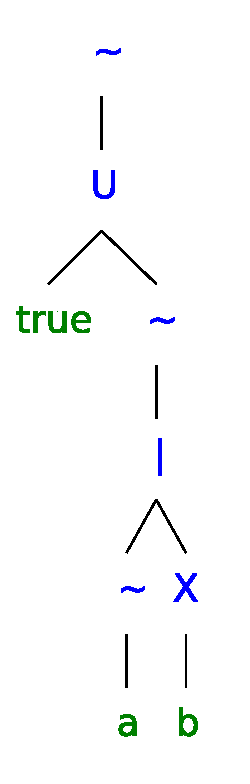
\includegraphics[height=15em, width=7.5em]{images/formula-syntax-tree}
	\caption{The syntax tree generated for the formula $"G(a \thicksim Xb)"$. Symbols are in green while operators are in blue.}
	\label{fig:formula-syntax-tree}
\end{figure}
Finally, as in the \texttt{MyLexer} class, we have to handle errors defining a specific method.

\LTLfToDFA can be used just for the parsing phase of an 	\LTLf formula as shown in Listing \ref{code:ltlf2dfa-only-parsing}.
\begin{lstlisting}[language=Python, style=Python, label={code:ltlf2dfa-only-parsing}, caption={How to use only the parsing phase of \LTLfToDFA.}]
from ltlf2dfa.Parser import MyParser

formula = "G(a->Xb)"
parser = MyParser()
parsed_formula = parser(formula)

print(parsed_formula) # syntax tree as tuple of tuples
\end{lstlisting}
\subsection{Translator.py}
The \texttt{Translator.py} module contains the majority of APIs that the \LTLfToDFA package exposes. Indeed, this module consists of a \texttt{Translator} class which concerns the core feature of the package: the translation of an \LTLf  formula into a \DFA. Since the package takes advantage of the \MONA tool for the formula conversion, the \texttt{Translator} class has to translate first the given formula into the syntax recognized by \MONA, then create the input program for \MONA and, finally, invoke \MONA to get back the resulting \DFA in the Graphviz\footnote{Graphviz is open source graph visualization software. For further details see \href{https://www.graphviz.org}{https://www.  .org}} format. 
The main methods of the \texttt{Translator} class are:
\begin{itemize}
\item \texttt{translate()}, which starting from the formula syntax tree generated (Figure \ref{fig:formula-syntax-tree}) in the parsing phase translates it into a string using the syntax of \MONA;
\item \texttt{createMonafile(flag)}, which, as the name suggests, creates the program \textit{.mona} that will be given as input to \MONA. The flag parameter is going to be \texttt{True} of \texttt{False} whether we need to compute also \declare  assumptions or not;
\item \texttt{invoke\_mona()}, which invokes \MONA in order to obtain the \DFA.
\end{itemize}
Now we will go into details of the methods stated above showing their implementation.
\subsubsection{The \texttt{translate} method}
The \texttt{translate} method is a crucial step towards reaching a good result and performance. Formally, the translation procedure from an \LTLf formula to the \MONA syntax is done passing through \FOL as shown in \ref{eq:translation-procedure}.
\begin{equation}\label{eq:translation-procedure}
\textsc{LTL}_f \rightarrow \textsc{FOL} \rightarrow \textsc{MONA}
\end{equation}
The former translation from \LTLf to \FOL is done accordingly to \citep{de2013linear}, while the latter follows from \citep{monamanual2001}.
In Listing \ref{code:ltlf2dfa-translate-method} we can see the translation's implementation. Three dots $\dots$ represent omitted code.
\begin{lstlisting}[language=Python, style=Python, escapechar = £,  label={code:ltlf2dfa-translate-method}, caption={The \texttt{translate} method.}]
import ...

class Translator:
    ...
    
    def translate(self):
        self.translated_formula = translate_bis(self.parsed_formula, \
        var='v_0')+";\n"

   ...

def translate_bis(formula_tree, var):£\label{line:translate_bis}£
    if type(formula_tree) == tuple:
        #enable this print to see the tree pruning
        # print(self.parsed_formula)
        # print(var)
        if formula_tree[0] == '&':
            # print('computed tree: '+ str(self.parsed_formula))
            if var == 'v_0':
                a = translate_bis(formula_tree[1], '0')
                # a = translate_bis(self.parsed_formula[1], '0')
                b = translate_bis(formula_tree[2], '0')
            else:
                a = translate_bis(formula_tree[1], var)
                b = translate_bis(formula_tree[2], var)
            if a == 'false' or b == 'false':
                return 'false'
            elif a == 'true':
                if b == 'true': return 'true'
            elif b == 'true': return a
            else: return '('+a+' & '+b+')'
        elif formula_tree[0] == '|':
            # print('computed tree: '+ str(self.parsed_formula))
            if var == 'v_0':
                a = translate_bis(formula_tree[1], '0')
                b = translate_bis(formula_tree[2], '0')
            else:
                a = translate_bis(formula_tree[1], var)
                b = translate_bis(formula_tree[2], var)
            if a == 'true' or b == 'true':
                return 'true'
            elif a == 'false':
                if b == 'true': return 'true'
                elif b == 'false': return 'false'
                else: return b
            elif b == 'false': return a
            else: return '('+a+' | '+b+')'
        elif formula_tree[0] == '~':
            # print('computed tree: '+ str(self.parsed_formula))
            if var == 'v_0': a = translate_bis(formula_tree[1], '0')
            else: a = translate_bis(formula_tree[1], var)
            if a == 'true': return 'false'
            elif a == 'false': return 'true'
            else: return '~('+ a +')'
        elif formula_tree[0] == 'X':
            # print('computed tree: '+ str(self.parsed_formula))
            new_var = _next(var)
            a = translate_bis(formula_tree[1],new_var)
            if var == 'v_0':
                return '('+ 'ex1 '+new_var+': '+ new_var +' = 1 '+ '& '+ \
                a +')'
            else:
                return '('+ 'ex1 '+new_var+': '+ new_var +' = '+ var + \
                ' + 1 '+ '& '+ a +')'
        elif formula_tree[0] == 'U':
            # print('computed tree: '+ str(self.parsed_formula))
            new_var = _next(var)
            new_new_var = _next(new_var)
            a = translate_bis(formula_tree[2],new_var)
            b = translate_bis(formula_tree[1],new_new_var)

            if var == 'v_0':
                if b == 'true': return '( '+ 'ex1 '+new_var+': 0 <= '+ \
                new_var+' & '+ new_var+' <= max($) & '+ a +' )'
                elif a ==  'true': return '( '+ 'ex1 '+new_var+': 0 <= '+ \
                new_var+' & '+new_var+' <= max($) & all1 '+ \
                new_new_var+': 0 <= '+new_new_var+' & '+ \
                new_new_var+' < '+new_var+' => '+b+' )'
                elif a == 'false': return 'false'
                else: return '( '+ 'ex1 '+new_var+': 0 <= '+new_var+ \
                ' & '+new_var+' <= max($) & '+ a +' & all1 '+ \
                new_new_var+': 0 <= '+new_new_var+' & '+ \
                new_new_var+' < '+new_var+' => '+b+' )'
            else:
                if b == 'true': return '( '+ 'ex1 '+new_var+': '+var+ \
                ' <= '+new_var+' & '+new_var+' <= max($) & '+ a +' )'
                elif a ==  'true': return '( '+ 'ex1 '+new_var+': '+var+ \
                ' <= '+new_var+' & '+new_var+' <= max($) & all1 '+ \ 
                new_new_var+': '+var+' <= '+new_new_var+' & '+ \ 
                new_new_var+' < '+new_var+' => '+b+' )'
                elif a == 'false': return 'false'
                else: return '( '+ 'ex1 '+new_var+': '+var+' <= '+ \ 
                new_var+' & '+new_var+' <= max($) & '+ a + \
                ' & all1 '+new_new_var+': '+var+' <= '+new_new_var+\
                ' & '+new_new_var+' < '+new_var+' => '+b+' )'
        elif formula_tree[0] == 'Y':
            # print('computed tree: '+ str(self.parsed_formula))
            new_var = _next(var)
            a = translate_bis(formula_tree[1],new_var)
            if var == 'v_0':
                return '('+ 'ex1 '+new_var+': '+ new_var + \
                ' = max($) - 1 '+ '& max($) > 0 & '+ a +')'
            else:
                return '('+ 'ex1 '+new_var+': '+ new_var + \
                ' = '+ var + ' - 1 '+ '& '+new_var+' > 0 & '+ a +')'
        elif formula_tree[0] == 'S':
            # print('computed tree: '+ str(self.parsed_formula))
            new_var = _next(var)
            new_new_var = _next(new_var)
            a = translate_bis(formula_tree[2],new_var)
            b = translate_bis(formula_tree[1],new_new_var)

            if var == 'v_0':
                if b == 'true': return '( '+ 'ex1 '+new_var+': 0 <= '+ \ 
                new_var+' & '+new_var+' <= max($) & '+ a +' )'
                elif a ==  'true': return '( '+ 'ex1 '+new_var+ \
                ': 0 <= '+new_var+' & '+new_var+ \
                ' <= max($) & all1 '+new_new_var+': '+new_var+' < '+ \ 
                new_new_var+' & '+new_new_var+' <= max($) => '+b+' )'
                elif a == 'false': return 'false'
                else: return '( '+ 'ex1 '+new_var+': 0 <= '+ \ 
                new_var+' & '+new_var+' <= max($) & '+ a + \
                ' & all1 '+new_new_var+': '+new_var+' < '+ \
                new_new_var+' & '+new_new_var+' <= max($) => '+b+' )'
            else:
                if b == 'true': return '( '+ 'ex1 '+new_var+ \ 
                ': 0 <= '+new_var+' & '+new_var+' <= max($) & '+ a +' )'
                elif a ==  'true': return '( '+ 'ex1 '+new_var+ \
                ': 0 <= '+new_var+' & '+new_var+' <= '+var+ \
                ' & all1 '+new_new_var+': '+new_var+' < '+ \
                new_new_var+' & '+new_new_var+' <= '+var+' => '+b+' )'
                elif a == 'false': return 'false'
                else: return '( '+ 'ex1 '+new_var+': 0 <= '+ \ 
                new_var+' & '+new_var+' <= '+var+' & '+ a +' & all1 '+ \ 
                new_new_var+': '+new_var+' < '+new_new_var+' & '+ \ 
                new_new_var+' <= '+var+' => '+b+' )'
    else:
        # handling non-tuple cases
        if formula_tree[0] == 'T': return 'true'
        elif formula_tree[0] == 'F': return 'false'

        # enable if you want to see recursion
        # print('computed tree: '+ str(self.parsed_formula))

        # BASE CASE OF RECURSION
        else:
            if formula_tree.isalpha():
                if var == 'v_0':
                    return '0 in '+ formula_tree.upper()
                else:
                    return var + ' in ' + formula_tree.upper()
            else:
                return var + ' in ' + formula_tree

def _next(var):
    if var == '0': return 'v_1'
    else:
        s = var.split('_')
        s[1] = str(int(s[1])+1)
        return '_'.join(s)
\end{lstlisting}
As we can see, the \texttt{translate} method is actually very simple. In fact, it just calls the \texttt{translate\_bis} function (line \ref{line:translate_bis}) to perform the proper translation. The function works in a recursive fashion taking as input the parsed formula and a variable and outputting a string containing the result. Obviously, when an instance of the \texttt{Translator} class is created the input formula is checked to have either only future or past operators.
The base case of the recursion handles the translation of symbols as they are the leaves of the syntax tree composed in the parsing phase (Figure \ref{fig:formula-syntax-tree}). On the other hand, the recursive step regards the handling of operators (non leaf components of the syntax tree) which are in our case $\lAND$, $\lOR$, $\NOT$, \Next, $\lUntil$, \Yesterday, $\Since$. During the translation, we simplify the resulting formula by avoiding pieces of the expression that are logically \texttt{True} or \texttt{False}. This simplification has two main advantages. First, it substantially reduces the length of the resulting formula, improving its readability. Second, it increases the computation performances of \MONA.
Additionally, since the \MONA syntax requires the declaration of the free variables, the \texttt{translate\_bis} function has to compute also the appriopriate free variables declaration. In this terms, the translation function uses the \texttt{\_next} function to compute the next variable each time is needed.

\subsubsection{The \texttt{createMonafile} method}
The \texttt{createMonafile} method is employed to write the program \textit{.mona} and save it in the main directory. It takes as input a boolean flag that, as stated before, stands for indicating whether one would like to compute and add the \declare assumption or not. In particular, in formal logic, as stated in \citep{DeGiacomo:2014:RLF:2893873.2894033}, the \declare assumption is expressed as in \ref{eq:declare-ass}.
\begin{equation}\label{eq:declare-ass}
\Always (\bigvee_{a \in \P} a) \lAND \Always (\bigwedge_{a,b \in \P, a \neq b} a \rightarrow \NOT b) 
\end{equation}
It consists essentially in two parts joined by the $\lAND$ operator. The former indicates that it is always true that at each point in time only one symbol is $\true$, while the latter means that always for each couple of different symbols in the formula if one is $\true$ the other must be $\false$.
The practical part can be seen in Listing \ref{code:ltlf2dfa-createmona-method}.
\begin{lstlisting}[language=Python, style=Python, escapechar = £, label={code:ltlf2dfa-createmona-method}, caption={The \texttt{createMonafile} method.}]
...
    def compute_declare_assumption(self):£\label{line:declare-ass-method}£
        pairs = list(it.combinations(self.alphabet, 2))

        if pairs:
            first_assumption = "~(ex1 y: 0<=y & y<=max($) & ~("
            for symbol in self.alphabet:
                if symbol == self.alphabet[-1]: first_assumption += \ 
                'y in '+ symbol +'))'
                else : first_assumption += 'y in '+ symbol +' | '

            second_assumption = "~(ex1 y: 0<=y & y<=max($) & ~("
            for pair in pairs:
                if pair == pairs[-1]: second_assumption += '(y notin '+ \
                pair[0]+' | y notin '+pair[1]+ ')));'
                else: second_assumption += '(y notin '+ pair[0]+ \
                ' | y notin '+pair[1]+ ') & '

            return first_assumption +' & '+ second_assumption
        else:
            return None

    def buildMonaProgram(self, flag_for_declare):£\label{line:build-mona-program}£
        if not self.alphabet and not self.translated_formula:
            raise ValueError
        else:
            if flag_for_declare:
                if self.compute_declare_assumption() is None:
                    if self.alphabet:
                        return self.headerMona + \
                        'var2 ' + ", ".join(self.alphabet) + ';\n' + \
                         self.translated_formula
                    else:
                        return self.headerMona + self.translated_formula
                else: return self.headerMona + 'var2 ' +\
                 ", ".join(self.alphabet) + ';\n' + \
                 self.translated_formula + \
                 self.compute_declare_assumption()
            else:
                if self.alphabet:
                    return self.headerMona + 'var2 ' +\
                     ", ".join(self.alphabet) + ';\n' + \
                     self.translated_formula
                else:
                    return self.headerMona + self.translated_formula

    def createMonafile(self, flag):
        program = self.buildMonaProgram(flag)
        try:
            with open('./automa.mona', 'w+') as file:
                file.write(program)
                file.close()
        except IOError:
            print('Problem with the opening of the file!')
...            
\end{lstlisting}
As shown in the code, the \texttt{createMonafile} method calls another method, the \texttt{buildMonaProgram} (line \ref{line:build-mona-program}), which literally builds the \textit{.mona} program by joining all pieces that should belong to it. Instead, regarding the \declare assumption, if needed, it is added to the \textit{.mona} program directly translated through \texttt{compute\_declare\_assumption} method at line \ref{line:declare-ass-method}.
\subsubsection{The \texttt{invoke\_mona} method}
Finally, the \texttt{invoke\_mona} method is the one that executes the \MONA compiled executable giving it the \textit{.mona} program. Consequently, the \DFA resulting from the computation of \MONA will be stored in the main directory. As stated in \ref{sec:intro}, the \LTLfToDFA package requires \MONA to be installed. Indeed, without this requirements the \texttt{invoke\_mona} method will raise an error. The implementation can be seen in Listing \ref{code:ltlf2dfa-invokemona-method}.
\begin{lstlisting}[language=Python, style=Python, escapechar = £, label={code:ltlf2dfa-invokemona-method}, caption={The \texttt{invoke\_mona} method.}]
...
    def invoke_mona(self, path='./inter-automa'):
        if sys.platform == 'linux':
            package_dir = os.path.dirname(os.path.abspath(__file__))
            mona_path = pkg_resources.resource_filename('ltlf2dfa','mona')
            if os.access(mona_path, os.X_OK):  #check if mona is executable
                try:
                    subprocess.call(package_dir+'/./mona -u -gw ' + \
                    './automa.mona > ' + path + '.dot', shell=True)
                except subprocess.CalledProcessError as e:
                    print(e)
                    exit()
                except OSError as e:
                    print(e)
                    exit()
            else:
                print('[ERROR]: MONA tool is not executable...')
                exit()
        else:
            try:
                subprocess.call('mona -u -gw ./automa.mona > ' + path + \
                '.dot', shell=True)
            except subprocess.CalledProcessError as e:
                print(e)
                exit()
            except OSError as e:
                print(e)
                exit()
...            
\end{lstlisting}
To the execute of the \MONA tool we have leveraged the built-in module \texttt{subprocess} that enables to spawn new processes, connect to their input/output/error pipes, and obtain their return codes.

Unfortunately, the \DFA resulting from \MONA needs to be post-processed because of some extra states added for other purposes not relevant for us. This aspect will be better explained in the following subsection \ref{sec:dot-handler}. 
\subsection{DotHandler.py}\label{sec:dot-handler}
The \texttt{DotHandler} class has been created in order to manage separately and better the post-processing of the \DFA, in \textit{.dot} format, resulting from the computation of \MONA. Indeed, since \MONA has been developed for different purposes, its output has an additional initial state and transition that to our intent are completely meaningless. 

Additionally, the interaction with the \textit{.dot} format has been implemented thanks to the \texttt{dotpy} library (available on GitHub\footnote{https://github.com/Francesco17/dotpy}) developed for this specific purpose paying particular attention to performances.

As we can see in the implementation of the \texttt{DotHandler} class in Listing \ref{code:ltlf2dfa-dothandler}, the main methods are \texttt{modify\_dot} and \texttt{output\_dot}.
\begin{lstlisting}[language=Python, style=Python, escapechar = £, label={code:ltlf2dfa-dothandler}, caption={The \texttt{DotHandler} class.}]
from dotpy.parser.parser import MyParser
import os

class DotHandler:

    def __init__(self, path='./inter-automa.dot'):
        self.dot_path = path
        self.new_digraph = None

    def modify_dot(self):£\label{line:modifydot}£
        if os.path.isfile(self.dot_path):
            parser = MyParser()
            with open(self.dot_path, 'r') as f:
                dot = f.read()
                f.close()

            graph = parser(dot)
            if not graph.is_singleton():
                graph.delete_node('0')
                graph.delete_edge('init', '0')
                graph.delete_edge('0', '1')
                graph.add_edge('init', '1')
            self.new_digraph = graph
        else:
            print('[ERROR] - No file DOT exists')
            exit()

    def delete_intermediate_automaton(self):
        if os.path.isfile(self.dot_path):
            os.remove(self.dot_path)
            return True
        else:
            return False

    def output_dot(self, result_path='./automa.dot'):£\label{line:outputdot}£
        try:
            if self.delete_intermediate_automaton():
                with open(result_path, 'w+') as f:
                    f.write(str(self.new_digraph))
                    f.close()
            else:
                raise IOError('[ERROR] - Something wrong occurred in '+ \
                'the elimination of intermediate automaton.')
        except IOError:
            print('[ERROR] - Problem with the opening of the file %s!' \
            %result_path)
\end{lstlisting}
The former method at line \ref{line:modifydot} takes advantage of the APIs exposed by \texttt{dotpy}. Especially, it parses the \textit{.dot} file output of \MONA (Figure \ref{fig:mona-output}), deletes the starting node $0$ and the edge from node $0$ to node $1$ and, finally, makes node $1$ initial. Consequently, the latter method at line \ref{line:outputdot} manages the output of the final post-processed \DFA (Figure \ref{fig:automa-post-processed}) and stores it in the main directory.
For instance, in Figure \ref{fig:pre-post-automaton} we can see graphically what is the outcome of the post-processing of the automaton corresponding to the formula $\varphi = \Always (a \rightarrow \Next b)$.
\begin{figure}[h]
\centering
\begin{subfigure}{.5\textwidth}
  \centering
  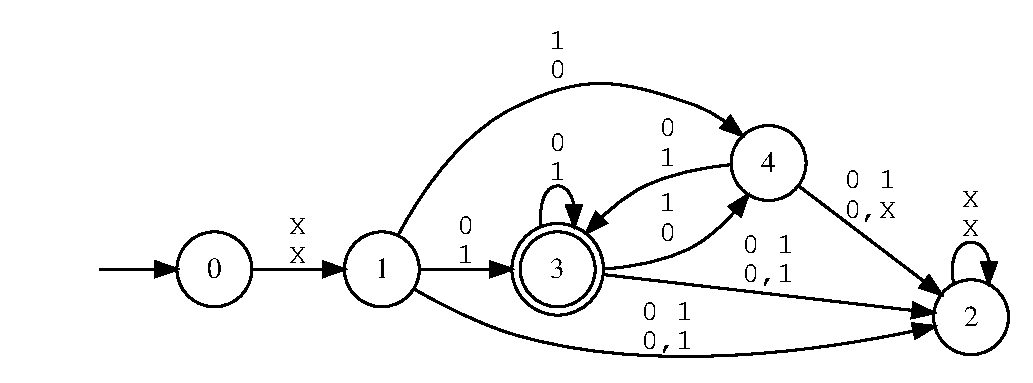
\includegraphics[width=\linewidth]{images/pre-automaton.eps}
  \caption{The \DFA output from \MONA}
  \label{fig:mona-output}
\end{subfigure}%
\begin{subfigure}{.5\textwidth}
  \centering
  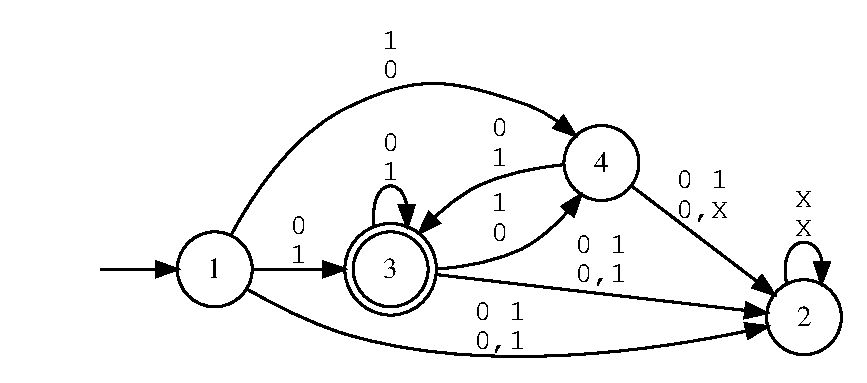
\includegraphics[width=\linewidth]{images/post-automaton.eps}
  \caption{The \DFA post-processed}
  \label{fig:automa-post-processed}
\end{subfigure}
\caption{Before and after \DFA post-processing}
\label{fig:pre-post-automaton}
\end{figure}
\section{Comparison with FLLOAT}
\section{Discussion}
In this chapter, we have presented the \LTLfToDFA Python package. We have also described the structure of the package, discussed in detail its implementation highlighting all the main features and, finally, seen how it performs with respect to time and memory relatively to the FLLOAT Python package.



















	\chapter{Janus}
In this chapter, we will illustrate how our tool \LTLfToDFA presented in Chapter \ref{ch:ltlf2dfa} can be efficiently employed in the field of Business Process Management, with particular attention to Process Mining. First of all, we will formally describe the theoretical framework of declarative process mining, introducing a new theorem that generalizes the concept of separated formulas only for \declare constraints. Then, in this context, we will thoroughly describe the implementation of the Janus algorithm \citep{cecconi2018interestingness} for computing the interestingness degree of traces in real event logs. Finally, we will provide such a computation for a real log as an example. 
\section{Declarative Process Mining}
In this section, we will present the theoretical framework of Business Process Management focusing our attention to declarative process mining. We will extend what described in Chapter \ref{ch:theory} providing all additional concepts, definitions and theorems necessary to clearly understand the context.

Business Process Management (BPM) deals with discovering, modeling, analyzing and managing business processes in order to measure their productivity and to improve their performance. These tasks are carried out thanks to logging facilities that, nowadays, all BPM systems have. The extraction and the validation of temporal constraints from event logs (i.e. multi-sets of finite traces) are techniques consisting declarative process mining \citep{montali2010declarative}. Temporal constraints are expressed using \LTLf and/or \PLTL and refers to activities present in traces. In the following, we will formally introduce what event logs and \declare \citep{pesic2008constraint} are. Another important aspect to notice is that these constraints are meant to be checked upon the activation satisfying specific conditions. For these reasons, they are referred as \emph{reactive constraints}.
\paragraph{Event Logs}
The event log is a collection of meaningful data that is the entry point for the consequent process mining. Formally, we consider this meaningful data expressed as a multiple traces containing a sequence of events belonging to the alphabet of symbols $\Sigma$. A single trace can be represented as $t = \tup{e_1,e_2,\dots,e_n}$ where $e_i$ is the event occurring at instant $i$ and $n \in \mathbb{N}$ is the length of the trace $t$.  Now, we can give the following definition:
\begin{definition}
An event log $\L$ is defined as $\L = \{t_1,\dots,t_m\} \in \mathbb{M} (\Sigma^*)$ is a multi-set of traces $t_j$ with $1 \le j \le m$, where $m \in \mathbb{N}$.
\end{definition}
To better indicate the \textit{multiplicity} of traces in $\L$, we can denote it as a superscript compacting the notation. For example, $t_{2}^{10}$ stands for trace $t_2$ occurs $10$ times in $\L$.
\begin{example}\label{ex:traces}
$\L = \{t_{1}^{25},t_{2}^{10},t_{3}^{15},t_{4}^{20},t_{5}^{5},t_{6}^{10}\}$ is an event log of $85$ traces, defined over the alphabet $\Sigma = \{a,b,c,\dots, i \} $. In $ \L $ we have the following traces:
\begin{align*}
t_1 &= \tup{d,f,a,f,c,a,f,b,a,f}\\
t_2 &= \tup{f,e,d,c,b,a,g,h,i}\\
t_3 &= \tup{a,d,a,a,a,a,a,a,a,a,a,a,a,a,a,a,a,a,a,a,a,c}\\
t_4 &= \tup{d,b,a,e}\\
t_5 &= \tup{a,d,a,c,a}\\
t_6 &= \tup{b,c,d,e}
\end{align*}
\end{example}
Furthermore, the event $e_i$ occurring at instant $i$ is denoted by $t(i)$, whereas the segment of $t$ (i.e. the sub-trace) ranging from instant $i$ to instant $j$, where $1 \le i \le j \le n$ is denoted by $t_{[i:j]}$.

Apart from the formal model of event logs, we have real-world event logs that are logs with real data coming from different kind of data sources (e.g. databases, transaction logs, audit log, etc.). All available tools are evaluated against real-world logs. In practice, as we will see in the Section \ref{sec:janus-implementation}, the main way of representing real logs is the XES Standard\footnote{http://www.xes-standard.org}, which is based on the well known XML.
\paragraph{\declare}
\declare is a language concerning declarative process modeling \citep{pesic2008constraint} and consisting of standard templates based on \citep{dwyer1999patterns} that was introduced to simplify the complexity of constraints semantics. Indeed, \declare constraints are expressed in \LTLf, but we will extend \LTLf with Past temporal operators (\LTLp) for capturing also past modalities. In Figure \ref{fig:declare-constraints}, we can see what are the corresponding \LTLf or \LTLp formulas for the most important \declare constraints. 
\begin{figure}[h]
\centering
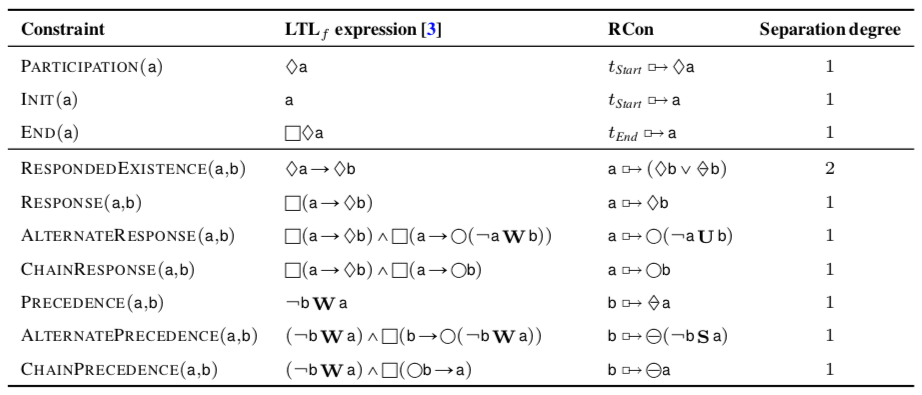
\includegraphics[width=\textwidth]{images/declare-constraints}
\caption{The most important \declare constraints expressed as \LTLf/\PLTL formulas and \emph{reactive constraints.}}
\label{fig:declare-constraints}
\end{figure}
Parameters in a template define tasks and they occurs as events in traces. In Example \ref{ex:declare-examples} we provide a glimpse of \declare patterns.
\begin{example}\label{ex:declare-examples}
Interesting \declare templates \citep{maggi2013knowledge}
\begin{itemize}
\item \textsc{Precedence}(a,b) means \emph{if b occurs then a occurs before b}.
\item \textsc{Responce}(a,b) means \emph{if a occurs then eventually b occurs after a}.
\item \textsc{ChainPrecedence}(a,b) means \emph{the occurrence of b imposes a to occur immediately before}.
\item \textsc{AlternateResponce}(a,b) means \emph{if a occurs then eventually
b occurs after a without other occurrences of a in between}.
\end{itemize}
\end{example}
In addition, one can create his own 	\declare patterns tailored for his purposes. In this way, the \declare standard template can be customized.

A given \declare constraint is verified over traces and those traces \emph{satisfy} it if they do not \emph{violate} it. Here, it is important to notice that these constraints are prone to the principle of \textit{ex falso quod libet}, namely they can be satisfied even without being activated. This represents a big issue for process mining because mining techniques might misunderstand the actual behavior of a process. The solution to this problem is to compute whether a constraint is satisfied or not only upon activation. However, we will see later how to overcome this problem in the Section \ref{sec:janus}.

Now, we give some definitions:
\begin{definition}\citep{gabbay1989declarative}\label{def:pure-temp-formula}
Given an \LTLp formula $\varphi$, we call it \emph{pure past} formula ($\varphi^\blacktriangleleft$) if it consists of only past operators; \emph{pure present} formula ($\varphi^\blacktriangledown$) if it has not any temporal operators; \emph{pure future} formula ($\varphi^\blacktriangleright$) if it consists of only future operators.
\end{definition}
\begin{example}\label{ex:pure-formulas-examples}
Pure formulas:
\begin{itemize}
\item $\boxminus(a \Rightarrow \Once b)$ is a \textbf{pure past} formula;
\item $a \Rightarrow (b \lAND c)$ is a \textbf{pure present} formula
\item $\Box(a \Rightarrow \Next b)$ is a \textbf{pure future} formula
\end{itemize}
\end{example}
The separation of an \LTLp formula to pure past/present/future formulas allows to conduct the analysis on sub-traces (i.e. one referring to the past and the other referring to the future) upon the activation. This is also known as bi-directional on-line analysis. To this extent, we rely on the Separation Theorem stated as follows:
\begin{theorem}\citep{gabbay1989declarative}\label{th:separation-theorem}
Any propositional temporal formula $\varphi$ can be rewritten as a boolean combination of pure temporal formulas.
\end{theorem}
Therefore, following Theorem \ref{th:separation-theorem}, we can give the Definition of \textit{separated formula} as follows:
\begin{definition}\citep{cecconi2018interestingness}\label{def:separated-formula}
Let  $\varphi$ an \LTLp formula over $\Sigma$. A temporal separation is a function $\S: \textsc{ltl}p_f  \rightarrow 2^{\textsc{ltl}p_f \times \textsc{ltl}p_f 	\times \textsc{ltl}p_f}$ such that: $\S(\varphi) = \{(\varphi^{\blacktriangleleft},\varphi^{\blacktriangledown},\varphi^{\blacktriangleright})_1,\dots,\\(\varphi^{\blacktriangleleft},\varphi^{\blacktriangledown},\varphi^{\blacktriangleright})_m\}$ such that:
\begin{equation}\label{eq:separated-formulas}
\varphi \equiv \bigvee^{m}_{j=1} (\varphi^{\blacktriangleleft} \lAND \varphi^{\blacktriangledown} \lAND \varphi^{\blacktriangleright})_j
\end{equation}
where $\varphi^\blacktriangleleft$, $\varphi^\blacktriangledown$ and $\varphi^\blacktriangleright$ are pure formulas over $\Sigma$ as in Definition \ref{def:pure-temp-formula}.
\end{definition}
Notice that Equation \ref{eq:separated-formulas} is a disjunction of conjunction. Moreover, each triple consisting the image function of $\S(\varphi)$ is generally called \emph{separated formula}. In the following, we give an example of separated formula.
\begin{example}\label{ex:separated-formulas}
The separated formulas for $(\Yesterday a \lOR \Diamond b$):
\begin{align*}
(\Yesterday a \lAND True \lAND True)\bigvee(True \lAND True \lAND \Diamond b)
\end{align*}
\end{example}
PUT HERE THE NEW GENERALIZATION OF THE THEOREM

Since the Janus algorithm relies on the construction of the automata for separated \LTLp formulas, we will refer to notions explained previously in Section \ref{sec:formula-to-automa}. The crucial point is that given a separated \LTLp formula $\varphi$ we can build a minimum \DFA that \emph{accepts} all and only the traces satisfying formula $\varphi$.

In the following sections, we will describe in details the Janus approach giving fundamentals definitions and theorems. Then, we will illustrate the algorithm and its practical implementation.
\section{Janus}\label{sec:janus}
Declarative process modeling defines a list of \declare constraints to be satisfied during the execution of the process model. These constraints are of a reactive nature in the sense that the occurrence of some task bounds the occurrence of other activities. As anticipated in the previous Section, this kind of behavior might lead to the principle of \textit{ex falso quod libet}, namely a constraint can be satisfied even though it is never activated. Here, the Janus approach \citep{cecconi2018interestingness} solves this problem allowing the user to indicate the activation condition for the constraint directly in the constraint formula. In this way, constraints are activated only if the activation condition holds. Therefore, we can refer to these constraints as \textit{reactive constraints} (\rcon).
\begin{definition}
Given an alphabet $\Sigma$, let $\alpha \in \Sigma$ be an \emph{activation} and $\varphi$ be an \LTLp formula over $\Sigma$. A Reactive Constraint (\rcon) $\Psi$ is a pair $(\alpha, \varphi)$, denoted as $\Psi \doteq \alpha \boxright \varphi$
\end{definition}
\subsection{Algorithm}
\section{Implementation}\label{sec:janus-implementation}
\subsection{Package Structure}
\subsection{Classes}
\section{Summary}
	\chapter{DFAgame}
	\chapter{Conclusions and Future Work}\label{ch:conclusion}
Continue the introduction and possible future work
\section{Overview}
\section{Main Contributions}
\section{Future Works}
\section{Final Remarks}
	
%	\appendix 
%	\input{chapters/appendix-flloat}
%	\input{chapters/appendix-rltg}

	
	\backmatter
	\phantomsection
	
	\bibliography{bib.bib}
	

\end{document}